\section{Detaching enclosed meshes}
In biomedical problems, volume meshes are often constructed from multiple surfaces enclosed in another, where each surface represents an organ or piece of tissue. Due to their complicated shape and close proximity, it is common to obtain intersections between these surfaces. Even when each segmented mesh is individually free of self-intersections, additional intersections can arise when they are merged into a single mesh. This makes producing a volume mesh for FEM impossible. Some of the methods we introduced above to merge neighboring meshes can be applied here, but they would result in a single merged mesh, which is not usable for all applications. Also, one component would end up protruding through the other, which is not anatomically correct. And finally, for FEM solutions, each compartment needs to be assigned its own properties.

A better solution is to detach the intersecting meshes. If one mesh touches or slightly penetrates another, it may be sufficient to slightly shrink the inner mesh and/or enlarge the outer mesh. This can eliminate intersections while preserving the geometry of each surface. 

A different solution is to move the intersecting sections away from each other. We developed an algorithm to implement this using Open3d \cite{zhou2018open3dmodernlibrary3d}. The process begins by identifying watertight submeshes within the input mesh. One mesh is designated for editing (moving mesh), while the other remains stationary (reference mesh). The algorithm then selects vertices from the moving mesh whose distances to the reference mesh are below a specified threshold. These vertices are then repositioned so that their distance to the reference mesh is exactly equal to the threshold, which effectively eliminates intersections along the way. Needless to say, some loss of volume in the adjusted meshes is inevitable, along with slight alternations in shape. It is crucial to define an acceptable threshold for loss in each specific  case. Figure \ref{fig:sol2-2} shows the original and repaired mesh for a test case with one sphere enclosing and intersecting another. Our method produced geometrically correct meshes of reasonable quality. The outer sphere was left fully intact, while the inner sphere has a slightly distorted shape and smaller volume than the original. The algorithm was also tested on a mesh from MedShapeNet \cite{Li2025medshapenet}, with the results presented in the supplemental material. We aim to further improve this method to produce higher quality results.

\begin{figure}[h]
    \centering
    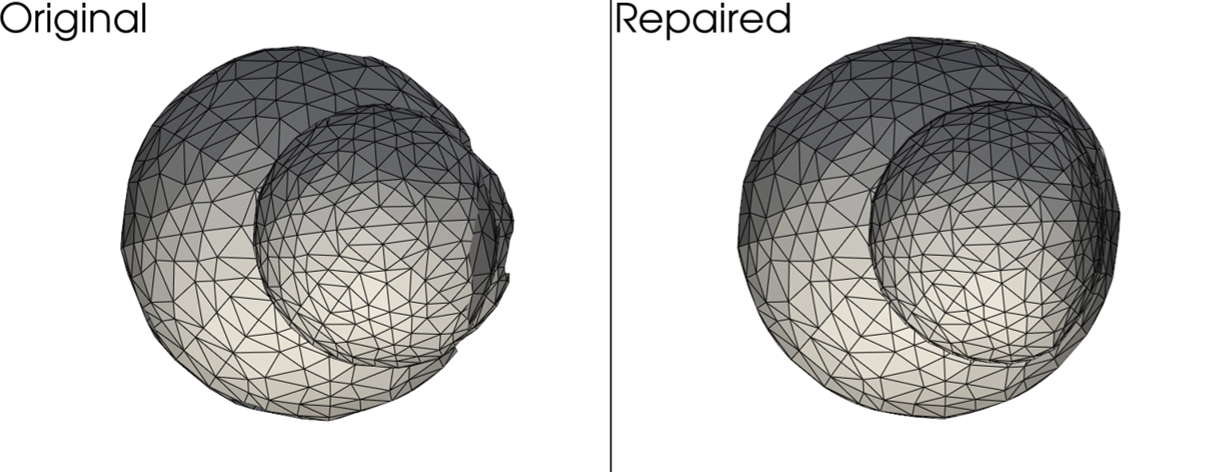
\includegraphics[ height=2.2cm]{../figures/new5.png}
    \caption{\textbf{Detaching enclosed meshes.} Original and repaired mesh for a test case with one sphere enclosed by another. The result is two distinct meshes without intersections.}
    \label{fig:sol2-2}
\end{figure}
\vspace{-1em}